\section{Brayton cycle}
\quad\, In this chapter, the different parts constituting the Brayton cycle have been well defined. The last part of the chapter will be devoted to the description and the performance analysis of the Brayton cycle considering various configurations.

The Brayton gas cycle (GT) is the most basic configuration where only four main elements are integrated within the cycle. First, there is the compressor (COMP) that will compress the ambient air. Then, the compressed air goes through the combustion chamber (CC) to increase its temperature. Finally, the exhaust gas from the combustion chamber are expanded through the turbine (TURB) to produce mechanical power. Part of this power is consumed by the compressor. The remaining is converted into electricity using an electrical generator. The gas cycle have been drawn on the following Figure \ref{fig:C3_BraytonGT}.

\begin{figure}[h]
\centering
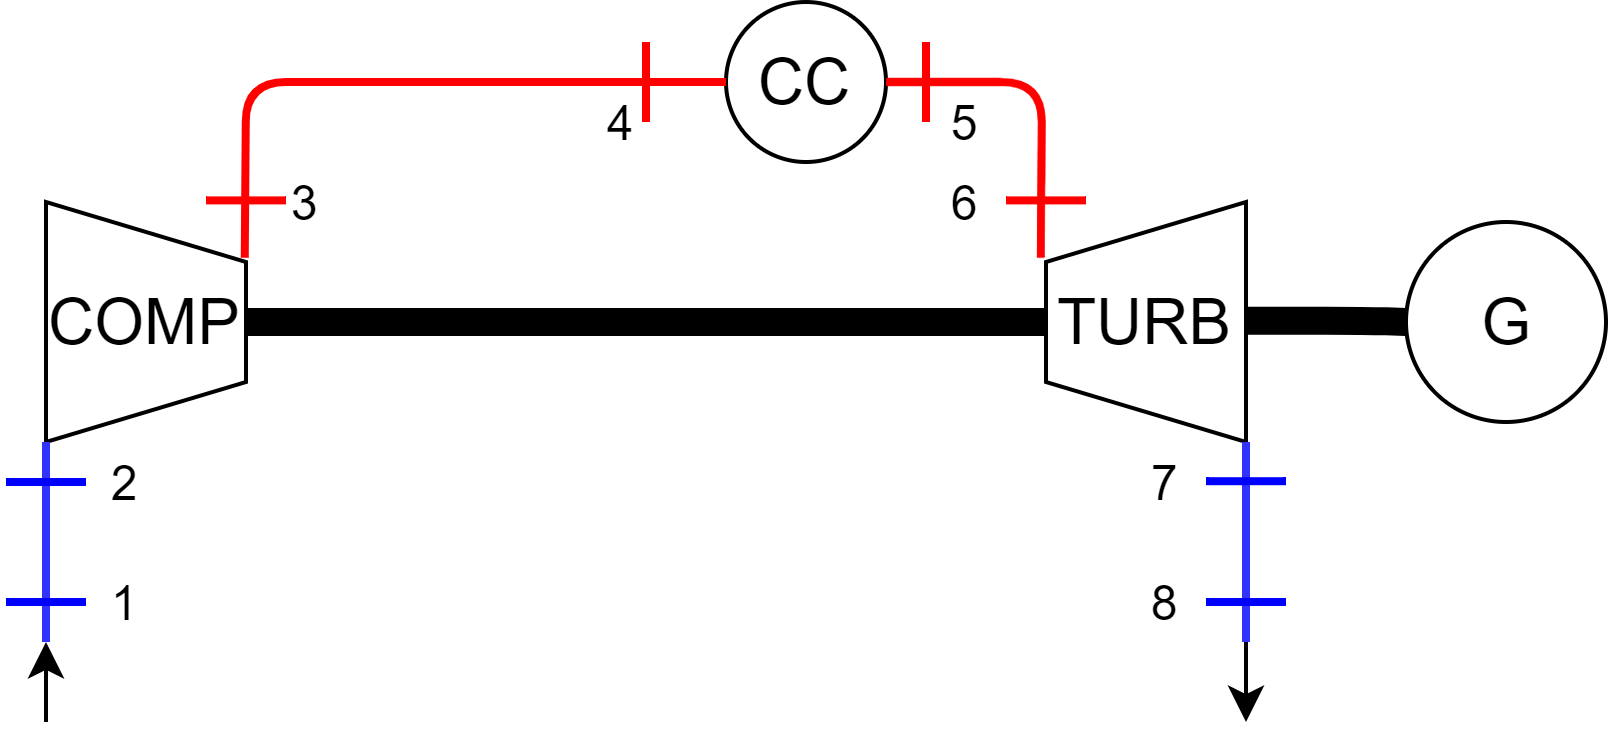
\includegraphics[width=0.5\textwidth]{GT}
\caption{Brayton gas cycle (GT)}
\label{fig:C3_BraytonGT}
\end{figure}

As illustrated, the cycle can be decomposed into 8 thermodynamic states.



\subsection{Thermodynamic diagram}
